% !TeX spellcheck = da_DK
Dette kapitel præsenterer en evaluering af projektets endelige løsning.
Først evalueres der på hvad robotten rent faktisk gør, hvorefter de to valgte sensormodeller (\cref{mapping:sensormodel}) for at finde ud af hvilken af de to der fungerer bedst.

\section{Observationer af robotten}
Efter gentagne kørsler med de to sensormodeller, har vi gjort vigtige observationer af hvor godt systemet fungerer.

Herunder beskrives de observationer, som har indvirkning på kvaliteten af det genererede kort.

\paragraph{Roterer og kører ikke præcist}
Et generelt problem, som kan observeres for alle kørsler, er hvordan robotten til tider placerer sig forkert i forhold til, hvor den bør placere sig inden en måling.
Dette giver dog ikke målinger det forkerte sted, da alle opdateringer af kortet sker efter robottens faktiske placering. 
Det betyder dog at det ikke altid er muligt, at foretage målinger hvor det ønskes.

\paragraph{Holder sig ikke altid indenfor den planlagte rute}
Når robotten følger den planlagte rute, skal den ideelt holde sig indenfor områder den ved der er ledige.
Dog betyder flere faktorer (for eksempel cellestørrelsen og at robotten ikke kører lige), at robotten ikke altid kan holde sig indenfor ruten.

\paragraph{Tager ikke højde for placering af sin bagende (og forende)}
Dette gælder især når den drejer, og når der foretages sensormålinger.
Når robotten drejer eller roterer, er der stor chance for at enten bagenden eller fronten af robotten rammer udenfor de kendte celler omkring den.
Robotten bakker tilbage for at tage højde for, at sensorerne ikke er placeret i midten ift. lokalisering, og kan også resultere i, at den kører udenfor de områder den kender til.

\paragraph{Sletter dele af kortet grundet forkerte sensormålinger}
Det er gentagne gange blevet observeret at dele af kortet, der ser fornuftigt ud, bliver ødelagt at gentagne fejlmålinger.
Dette kan betyde at robotten ikke længere kan nå frem til de områder, som er påvirket af fejlmålingerne.

\paragraph{Uendelig løkke}
Fejlmålinger kan også føre til en \textit{uendelig løkke}, hvilket henviser til at gentagne fejlmålinger kan 'fjerne' allerede kendte forhindringer fra kortet.
Sker det, og robotten ønsker at opdatere det \textit{nyopdagede} område (hvilket den ikke kan, da det er en fejl), så vil robotten blive ved med at forsøge at komme til det ufremkommelige område, ved at køre ind i forhindringen.
Da den aldrig kommer til den nye destination, men blot rammer forhindringen, vil det fortsætte med dette sålænge der er strøm på batteriet.

\paragraph{Kører ind i forhindringer}
At robotten kan risikere at ramme forhindringer, hænger sammen med alle ovenstående beskrivelser.
Dette sker således ved fejlmålinger, rotation og navigation.
For at forhindre dette sker, vil det være nødvendigt enten altid at tage afstandsmålinger i kørselsretningen, eller vha. en kontakt der aktiveres ved kontakt med et objekt.

\paragraph{}

På trods af disse svagheder, opnås der stadig resultater som stemmer overens med virkeligheden; altså hvordan testmiljøet ser ud.
Både banens kanter og forhindringer findes af robotten så den kan navigere rundt i området.

\section{Formål}
Formålet med denne test er at se hvilken sensormodel, der kommer frem til det mest præcise kort.
Dette er for at se om målsætningen beskrevet på side \pageref{problem:maalsaetning} er opfyldt.

\section{Vurderingsmål}
Da alle tests vil returnere et helt eller delvist udfyldt occupancy grid, vil sammenligningen gå ud fra dette.
Alle grids, som er resultat af en test, vil blive sammenlignet med et optimalt occupancy grid (lavet ud fra fysisk observation).
Ethvert grid (både test og optimalt) vil bestå af tre typer celler:
\begin{description}
\item[Optaget]{ er en celle, hvor der er en forhindring.}
\item[Fri]{ er en celle der er fri.}
\item[Ukendt]{ er en celle, hvor om der ikke er opnået viden.
For det optimale grid, vil det være celler inde i en større forhindring.
For et test grid, kan det være det samme som for det optimale, dog kan der også forekomme ukendte celler, som skulle have været enten frie eller optagede.}
\end{description}

\subsection{Sammenligning}
For enhver celle i et test grid, vil denne blive sammenlignet med den tilsvarende celle i det optimale grid.
Der vil være i alt 9 scenarier, da enhver celle har 3 tilstande.
I \cref{evaluering:sammenligning} kan resultatet af denne sammenligning ses.

\begin{table}[h]
\centering
\begin{tabular}{|l|c|c|c|}
\hline
Test \textbackslash~Optimalt & Optaget & Fri & Ukendt \\ \hline
Optaget & $+1$ & $-1$ & $0$ \\ \hline
Fri & $-1$ & $+1$ & $0$ \\ \hline
Ukendt & $-1$ & $-1$ & $0$ \\ \hline
\end{tabular}
\caption{Resultater for sammenligning af test grid celle og optimalt grid celle.}
\label{evaluering:sammenligning}
\end{table}

\subsection{Resultat}
Resultatet for et enkelt test grid vil være en akkumulering af sammenlignings-værdierne for cellerne.
Derved kommer der et enkelt tal for enhver test, hvorfor disse efterfølgende let kan sammenlignes.

\section{Test}\label{evaluering:test_beskrivelse}
Der bliver foretaget tre tests med hver sensormodel (\cref{mapping:sensormodel}).
I alle test benyttes ruteplanlægning beskrevet i \cref{ruteplanleagning}.
Robotten kører hen til et punkt og scanner to gange - dette foretages 75 gange.
Alle data bliver logget, så det er muligt at genskabe et kort udfra det.

\subsection{Opstilling}\label{evaluering:opstilling}
Testmiljøet er beskrevet i \cref{testmiljo}.
Selve opstillingen til testen kan ses på \cref{evaluering:emptyGrid}, her kan man desuden se robottens startposition, som er den samme i alle tests.

\begin{figure}[h]
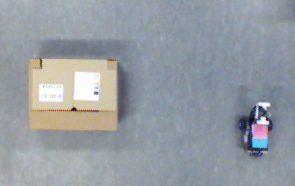
\includegraphics[width=\textwidth]{emptyGrid}
\caption{Forsøgsopstillingen inden hver test sættes i gang.}
\label{evaluering:emptyGrid}
\end{figure}

\subsection{Resultater}

\subsubsection*{Optimalt resultat}
For at kunne lave en sammenligning mellem resultater, skal hvert enkelt resultat først sammenlignes med det optimale, hvorefter afvigelsen kan måles og sammenlignes.

Det optimale grid består af i alt 555 markede celler; 110 optagede celler og 445 frie celler.
Det optimale grid kan ses i \cref{evaluering:optimaltgrid}.

\begin{figure}[h]
\begin{subfigure}[t]{.48\textwidth}
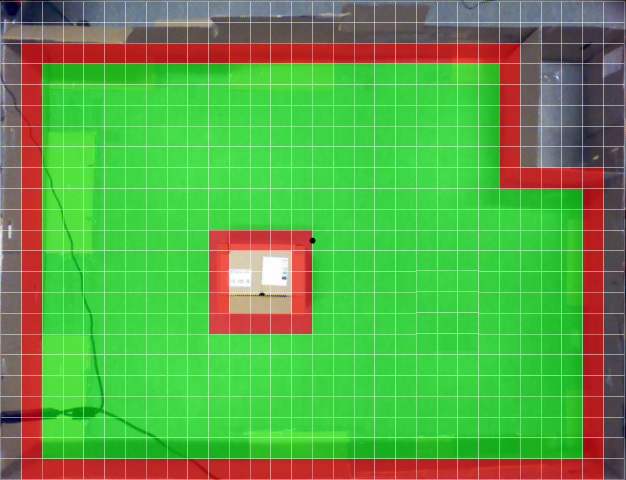
\includegraphics[width=\textwidth]{testresultater/optimalt}
\caption{Det optimale grid.}
\label{evaluering:optimaltgrid}
\end{subfigure}
\hfill
\begin{subfigure}[t]{.48\textwidth}
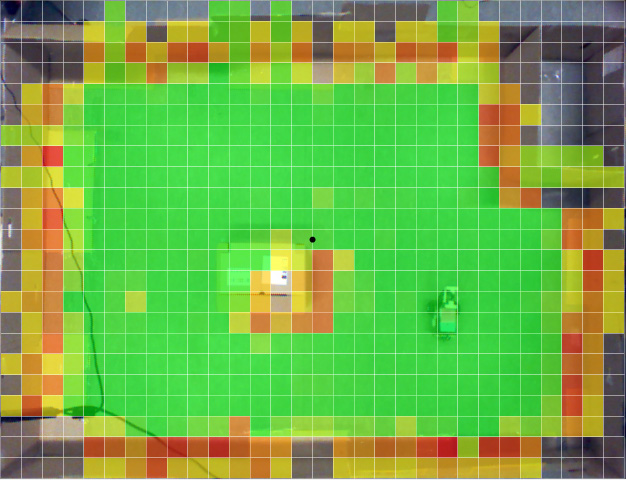
\includegraphics[width=\textwidth]{testresultater/gauss3}
\caption{Det bedste resultat (gausisk sensormodel).}
\label{evaluering:gauss3}
\end{subfigure}
\centering
\begin{subfigure}[b]{.48\textwidth}
\vspace{0.5em}
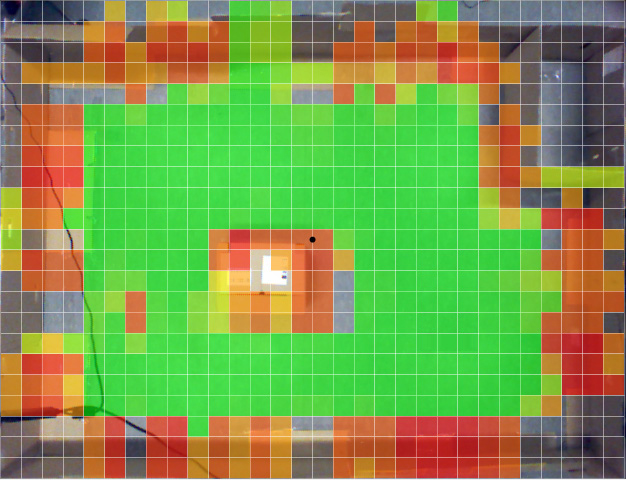
\includegraphics[width=\textwidth]{testresultater/simpel1}
\caption{Det bedste resultat med den simple sensormodel.}
\label{evaluering:simpel1}
\end{subfigure}
\caption{Det optimale grid kontra de bedste resultater.}
\label{evaluering:optvsbedst}
\end{figure}




\subsubsection*{Bedste resultat}
Det bedste resultat var for den 3. test med Gaussian Sensor Model.
Resultatet var 337 korrekte celler (ud af de 555 mulige), som det kan ses i \cref{evaluering:gauss3}. 
Det  bedste resultat med den simple sensormodel var den 1. test. 
Dette kan ses på \cref{evaluering:simpel1}.
Resultatet for denne var 193 korrekte celler.

\subsubsection*{Øvrige resultater}
De øvrige test-resultater kan ses i \cref{evaluering:testresultater}.
Her kan det ses at den Gaussiske sensor model giver klart det bedste resultat, og at resultaterne er nogenlunde konsistente hver især for de to modeller.

\begin{table}[h]
\centering
\begin{tabular}{|l|r|}
\hline
\textbf{Test \#} & \textbf{Resultat} \\ \hline \hline
Simpel, Test 1 & 193 \\ \hline
Simpel, Test 2 & 187 \\ \hline
Simpel, Test 3 & 193 \\ \hline \hline
Gaussisk, Test 1 & 297 \\ \hline
Gaussisk, Test 2 & 325 \\ \hline
Gaussisk, Test 3 & 337 \\ \hline
\end{tabular}
\caption{Oversigt over test-resultaterne.}
\label{evaluering:testresultater}
\end{table}

\subsubsection*{Konklusion}
Ud fra resultaterne kan det ses at den gaussiske model præsterer bedre end den simple sensormodel. 
Resultaterne for den simple model ligger omkring 190 mens resultaterne for den gaussiske liger omkring 300.

Ud fra kortene kan det dog ses at den simple finder kassen bedre end den gaussiske.
Som det ses på \cref{evaluering:gauss3} er kassens omrids kun markeret i nederste højre hjørne, mens den simple model på \cref{evaluering:simpel1} har har et større område der er markeret som optaget.
I praksis vil det betyde at selvom den gaussiske giver et mere præcist resultat er der en risiko for at den vil lave et kort hvor der er frie celler hvor der burde være optaget, hvilket kan få robotten til at køre ind i en væg.
